\chapter{Project Initiation}

\section{Introduction}

This chapter presents the overall context of the project and defines the environment in which it was developed. It introduces the host organization, outlines the problem being addressed, and reviews existing solutions together with their limitations. Based on this analysis, the proposed approach is presented and justified.

The chapter also specifies the system requirements, describes the technologies involved, and explains the development methodology adopted during the project. In addition, it summarizes the planning process through Agile sprints and provides a general overview of the system architecture.

Overall, this chapter lays the groundwork for the remainder of the report by clarifying the objectives, constraints, and design choices guiding the development of the system.

\section{Host Company Presentation}

This project was carried out as part of a final-year internship at \textbf{GExpertise}, a French engineering group specializing in topography, geospatial measurement, and digital modeling applied to construction and land development~\cite{gexpertise}.

\begin{figure}[htbp]
    \centering
    
\includegraphics[width=0.2\textwidth]{images/entreprise/LogoGexpertise.png}
    \caption{GExpertise Company Logo}
    \label{fig:gexpertise}
\end{figure}

Established in 2008, GExpertise builds upon a long professional heritage dating back to 1785, originating from a lineage of surveyors and geometers.

The company operates as a multidisciplinary organization structured around several engineering domains, including topography, construction engineering, real estate diagnostics, and geospatial data processing. It plays a central role in the acquisition, processing, and utilization of spatial data, supporting projects across the full lifecycle of buildings and infrastructure.

\subsection{Main Activity Domains}

GExpertise’s activities are organized into several complementary domains:

\begin{itemize}
    \item \textbf{Topography and Land Surveying:} \\
    This domain focuses on measurement, mapping, and land analysis, providing essential data for engineering and construction projects.

    \item \textbf{Building and Infrastructure Engineering (Bâtiment \& VRD):} \\
    It includes technical studies related to construction, infrastructure planning, and urban development.

    \item \textbf{Diagnostics and Real Estate Expertise:} \\
    The company offers diagnostic services to ensure compliance, risk assessment, and support for real estate operations.

    \item \textbf{BIM and GIS (SIG):} \\
    Advanced tools such as Building Information Modeling (BIM) and Geographic Information Systems (GIS) are used to structure and analyze spatial data.

    \item \textbf{Geospatial Data Acquisition and Processing:} \\
    Technologies such as drones, 3D scanning, and digital surveying tools are used to capture and transform spatial data into usable information.
\end{itemize}

The company’s mission is to measure, model, and structure the physical environment by delivering accurate and reliable data that supports decision-making. This involves the use of advanced digital tools such as GIS, BIM, and 3D reconstruction techniques.

GExpertise places strong emphasis on supporting clients, modeling complex environments, and ensuring the reliability of results. These principles are reinforced by values such as responsibility, engagement, and trust.

Operating in a context of continuous technological evolution, the company integrates digital innovation into traditional engineering practices to address modern challenges in infrastructure and urban development.

Within this environment, the internship provided an opportunity to contribute to a real-world project involving system design, geospatial processing, and real-time data handling. The development of the intelligent carpooling platform aligns with the company’s vision of leveraging data and digital technologies to improve operational efficiency.

\section{Problem Statement}

Daily commuting within corporate environments represents a significant challenge. The heavy reliance on private vehicles contributes to traffic congestion, increased transportation costs, and environmental impact.

Although carpooling offers a potential solution, existing approaches often lack flexibility and adaptability. In particular, matching users efficiently becomes difficult when their locations and schedules vary.

The problem addressed in this project can therefore be formulated as follows:

\textit{How can an intelligent, flexible, and scalable carpooling system be designed to efficiently match users within a real-world enterprise environment?}

\section{Project Objectives}

The objective of this project is to design and implement a carpooling platform adapted to enterprise needs.

To achieve this goal, the following objectives were defined:

\begin{itemize}
    \item Develop a ride-sharing system adapted to employee commuting behavior
    \item Design a matching mechanism based on route overlap
    \item Integrate machine learning techniques for commute prediction
    \item Enable real-time interaction between users
    \item Ensure a scalable and maintainable architecture
\end{itemize}

\section{Analysis of Existing Solutions}

Several carpooling platforms have been developed to address transportation challenges, including well-known solutions such as BlaBlaCar and Uber Pool.

However, these platforms are designed for public use, whereas the system proposed in this project targets an internal enterprise environment where all users belong to the same organization.

As a result, such platforms are considered indirect competitors. While they provide useful insights into ride-sharing mechanisms, they do not address enterprise-specific constraints.

Most existing systems rely on predefined routes and fixed pickup locations, which limits flexibility. Additionally, they operate in open environments where trust must be managed through external mechanisms such as ratings and verification systems.

In contrast, enterprise environments inherently provide a higher level of trust, since all users are verified members of the same organization.

\subsection{Comparative Analysis}

Table~\ref{tab:comparison} highlights the main differences between traditional carpooling systems and the proposed solution.

\begin{table}[H]
\centering
\renewcommand{\arraystretch}{1.3}
\begin{tabular}{|l|c|c|}
\hline
\textbf{Feature} & \textbf{Traditional Systems} & \textbf{Proposed System} \\
\hline
Matching basis & Fixed origin--destination points & Route-based trajectory overlap \\
\hline
Real-time updates & Limited or polling-based & WebSocket event-driven \\
\hline
Intelligence layer & None & ML-based commute prediction \\
\hline
Matching flexibility & Low (exact match required) & High (corridor-based proximity) \\
\hline
Enterprise integration & External trust mechanisms & Internal verified-user model \\
\hline
\end{tabular}
\caption{Comparison of Traditional Systems vs. Proposed System}
\label{tab:comparison}
\end{table}

The proposed system differs from existing approaches by introducing route-based matching, real-time communication, predictive intelligence, and internal trust management within the organization.

\section{Limitations of Existing Solutions}

The analysis highlights several limitations when traditional systems are applied to enterprise contexts:

\begin{itemize}
    \item Rigid matching based on fixed pickup locations
    \item Limited flexibility for diverse commuting routes
    \item Lack of adaptation to recurring travel patterns
    \item Dependence on external trust mechanisms
    \item Absence of enterprise-oriented coordination features
\end{itemize}

These limitations reduce the effectiveness of traditional carpooling systems in structured organizational environments.
\section{Proposed Solution}

To address the previously identified challenges, this work introduces an intelligent carpooling platform tailored for enterprise environments.

In contrast to public ride-sharing platforms, the system operates within a closed organizational setting. This context provides inherent advantages such as improved privacy, simplified identity verification, and a stronger level of trust among users belonging to the same organization.

The platform relies on a dynamic matching strategy based on route overlap analysis. Rather than constraining passengers to predefined pickup points, the system identifies feasible pickup locations along a driver’s route, which significantly increases matching opportunities while preserving route coherence.

In addition, a machine learning component is incorporated to analyze historical commuting data and detect recurring travel patterns. This enables predictive features that suggest relevant rides to users based on their behavior.

By combining deterministic geospatial processing with data-driven prediction, the system achieves a balance between accuracy, flexibility, and adaptability.

This approach differs from conventional carpooling systems that rely on fixed matching and passive interaction. By integrating route-based trajectory analysis, predictive intelligence, and real-time coordination, the platform transforms carpooling into a dynamic and context-aware system. The combination of deterministic matching, machine learning, and event-driven synchronization represents the core originality of the proposed solution.

\subsection{Advantages of the Proposed Solution}

Compared to existing platforms, the proposed system offers the following advantages:

\begin{itemize}
    \item Improved privacy through deployment within a closed enterprise environment
    \item Higher trust level due to verified users within the same organization
    \item Increased flexibility through route-based matching
    \item Adaptation to recurring commuting patterns
    \item Enhanced user experience through intelligent features
\end{itemize}

\section{Project Contributions}

This work contributes to the field of intelligent transportation systems through:

\begin{itemize}
    \item A route-based matching approach that increases flexibility compared to fixed-point systems
    \item A hybrid architecture combining deterministic algorithms and machine learning techniques
    \item An enterprise-oriented design leveraging internal trust and controlled access
    \item Integration of real-time communication mechanisms to improve interaction
\end{itemize}

These contributions differentiate the proposed system from traditional carpooling solutions.

\section{Requirements Specification}

\subsection{Functional Requirements}

The system provides the following functionalities:

\begin{itemize}
    \item User registration and secure authentication
    \item Profile management and personalization
    \item Ride creation, update, and cancellation
    \item Ride search and booking
    \item Intelligent matching between drivers and passengers
    \item Real-time notifications and communication
\end{itemize}

\subsection{Non-Functional Requirements}

The system must satisfy the following quality attributes:

\begin{itemize}
    \item \textbf{Scalability:} Support for an increasing number of users
    \item \textbf{Performance:} Efficient processing and low response time
    \item \textbf{Security:} Protection of user data and secure access control
    \item \textbf{Usability:} Intuitive and accessible user interface
    \item \textbf{Reliability:} Stable and consistent system behavior
\end{itemize}

\section{Technologies Used}

The system is built on a technology stack selected according to performance, scalability, and integration requirements.

\subsection{Backend Technology}

The backend is implemented using \textbf{Flask}, a lightweight Python web framework~\cite{flask}.

Flask was chosen for its simplicity and flexibility, enabling fine-grained control over system architecture and facilitating the integration of custom logic required for the intelligent matching mechanism. Furthermore, Python provides strong support for data processing and machine learning.

\subsection{Frontend Technology}

The frontend is developed using \textbf{Flutter}~\cite{flutter}.

Flutter allows the development of a single codebase for multiple platforms while maintaining performance and consistency. Its reactive architecture enables the creation of responsive interfaces suitable for real-time interaction.

\subsection{Database Management System}

The system uses \textbf{PostgreSQL}~\cite{postgresql} as its database management system.

PostgreSQL was selected for its robustness, scalability, and advanced querying capabilities, ensuring reliable data storage and integrity.

\subsection{Geospatial Services}

Geospatial processing relies on \textbf{OpenStreetMap (OSM)}~\cite{osm} and \textbf{OSRM}~\cite{osrm}.

These tools provide accurate route computation and efficient handling of geographic data, which are essential for implementing route-based matching.

\subsection{Real-Time Communication}

Real-time interaction is handled using \textbf{WebSocket} technology~\cite{websocket}.

WebSockets enable continuous bidirectional communication between the client and the server, allowing instant updates and synchronization. Unlike traditional request-response models, this approach maintains an open connection for real-time data exchange.

Within this system, WebSockets are used to deliver notifications, update ride status, and synchronize interactions between users, ensuring immediate feedback during system operations.

\subsection{Technology Selection Justification}

The selected technologies ensure a balance between performance, scalability, and flexibility. They support real-time communication, geospatial processing, and intelligent features, forming a solid foundation for the proposed system.
\section{Development Methodology}

The project followed an Agile development methodology based on the Scrum framework. Scrum structures work into time-boxed iterations called sprints, typically lasting two to four weeks, delivering potentially shippable product increments.

This methodology was selected due to its suitability for the project context:
\begin{itemize}
    \item \textbf{Iterative development:} Progressive system construction with regular validation
    \item \textbf{Continuous feedback:} Stakeholder input throughout the development lifecycle
    \item \textbf{Incremental delivery:} Functional features at regular intervals
    \item \textbf{Flexibility:} Accommodation of evolving requirements
    \item \textbf{Risk mitigation:} Early issue detection through frequent reviews
\end{itemize}

The main concepts of the Scrum methodology are illustrated in Figure~\ref{fig:scrum}.

\begin{figure}[htbp]
    \centering
    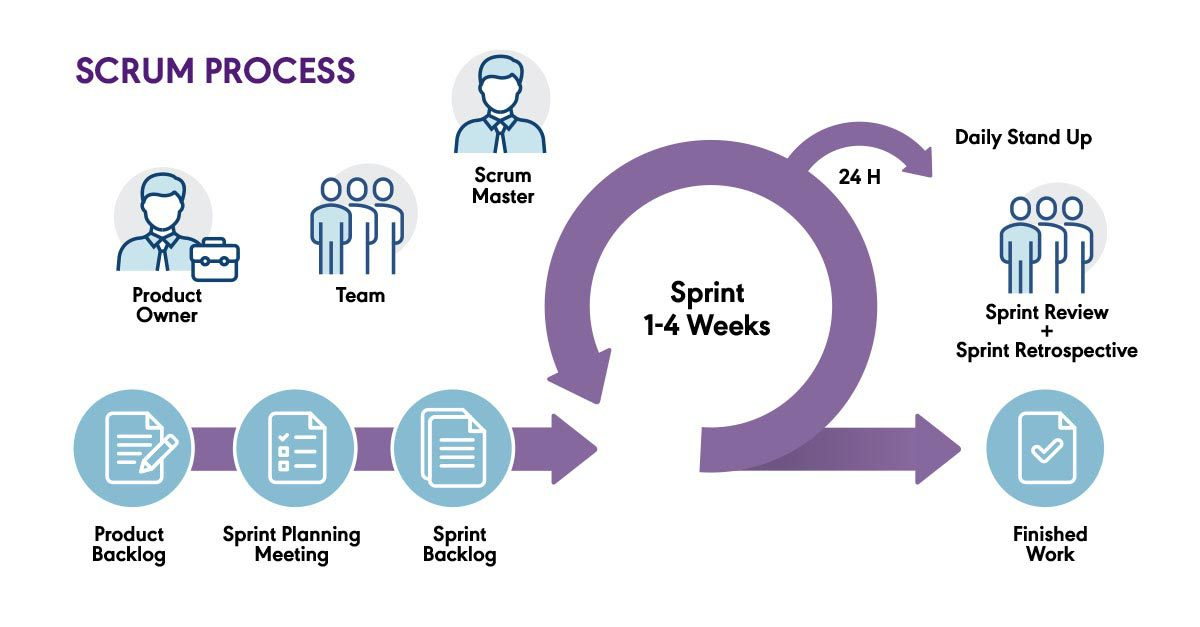
\includegraphics[width=0.75\textwidth]{images/methodology/scrum.jpg}
    \caption{Scrum Development Process}
    \label{fig:scrum}
\end{figure}

The methodology was applied through sprint planning, daily progress tracking, sprint reviews, and retrospectives. Validation activities were performed continuously at the end of each sprint, ensuring consistent quality and alignment with project objectives.

\section{Scrum Roles}

The Scrum framework defines three core roles, adapted to this professional internship context as follows:

\begin{itemize}
    \item \textbf{Product Owner:} The industrial supervisor from the host company, responsible for representing business stakeholders, defining project requirements, validating system increments, and ensuring the delivered solution creates measurable value for the enterprise.
    \item \textbf{Scrum Master:} The process facilitator responsible for organizing sprint planning and review sessions, monitoring progress, removing technical and organizational impediments, and ensuring strict adherence to Agile practices throughout the development lifecycle.
    \item \textbf{Development Team:} A collaborative development team composed of the intern working in coordination with technical supervisors and company mentors. This structure ensures continuous validation, code review, and knowledge transfer within a real engineering environment, while maintaining cross-functional responsibility for design, implementation, and quality assurance of each system increment.
\end{itemize}

\section{Product Backlog}

The Product Backlog represents the comprehensive set of features and user stories defining the complete system vision. It captures requirements from both end-users (collaborators) and administrative actors. Table~\ref{tab:backlog} presents the prioritized user stories for this project.

\begin{table}[!htbp]
\centering
\renewcommand{\arraystretch}{1.2}
\small
\begin{tabular}{|c|p{9cm}|c|}
\hline
\textbf{ID} & \textbf{User Story} & \textbf{Priority} \\
\hline
\multicolumn{3}{|c|}{\textbf{Core Features---Collaborator}} \\
\hline
US01 & As a collaborator, I want to register and authenticate securely to access the system & High \\
\hline
US02 & As a collaborator, I want to manage my profile and preferences & High \\
\hline
US03 & As a collaborator, I want to create and publish a ride offer with route details & High \\
\hline
US04 & As a collaborator, I want to search for available rides matching my needs & High \\
\hline
US05 & As a collaborator, I want to book a ride and receive confirmation & High \\
\hline
US06 & As a collaborator, I want to manage my bookings and ride history & High \\
\hline
\multicolumn{3}{|c|}{\textbf{Real-Time Features---Collaborator}} \\
\hline
US07 & As a collaborator, I want to receive real-time notifications about ride status & High \\
\hline
US08 & As a collaborator, I want to see live updates when bookings are confirmed or cancelled & Medium \\
\hline
\multicolumn{3}{|c|}{\textbf{Intelligent Features---Collaborator}} \\
\hline
US09 & As a collaborator, I want to be matched with optimal ride partners based on route overlap & High \\
\hline
US10 & As a collaborator, I want to receive ML-based commute suggestions based on my patterns & Medium \\
\hline
\multicolumn{3}{|c|}{\textbf{Administrative Features---Admin}} \\
\hline
US11 & As an admin, I want to monitor system activity and user engagement & Medium \\
\hline
US12 & As an admin, I want to view analytics on ride statistics and matching efficiency & Medium \\
\hline
US13 & As an admin, I want to manage users and freeze accounts when necessary & Medium \\
\hline
US14 & As an admin, I want to view system health and performance metrics & Low \\
\hline
\end{tabular}
\caption{Product Backlog -- User Stories by Actor and Feature Category}
\label{tab:backlog}
\end{table}

This Product Backlog represents the global system vision encompassing all required functionality. The detailed technical breakdown and sprint allocation will be presented in Chapter~3, where each user story is mapped to specific development iterations with corresponding use case diagrams, sequence diagrams, and implementation details.
\section{Backlog Structuring and Prioritization}

The Product Backlog was structured into six phases ensuring systematic progression from infrastructure to intelligent capabilities:

\begin{itemize}
    \item \textbf{Phase 1 -- Foundation (US01--US02):} Authentication and user management
    \item \textbf{Phase 2 -- Core Features (US03--US06):} Ride creation, search, and booking
    \item \textbf{Phase 3 -- Real-Time (US07--US08):} WebSocket communication and notifications
    \item \textbf{Phase 4 -- Intelligent Matching (US09):} Route-based geospatial matching
    \item \textbf{Phase 5 -- Machine Learning (US10):} Commute prediction based on patterns
    \item \textbf{Phase 6 -- Admin (US11--US14):} Monitoring and analytics
\end{itemize}

This sequencing respects architectural dependencies: real-time features require ride infrastructure; intelligent matching depends on operational data; machine learning requires accumulated patterns. Each sprint delivers a validated increment upon which subsequent work builds.

\section{Sprint Planning}

The development process was structured into seven sprints, each focusing on specific objectives over a total duration of approximately four months (around 17 weeks). This iterative approach allowed progressive system development, continuous validation, and effective management of project complexity. Table~\ref{tab:sprints} presents the detailed sprint planning.

\begin{table}[H]
\centering
\begin{tabular}{|c|c|p{4cm}|p{5cm}|}
\hline
\textbf{Sprint} & \textbf{Duration} & \textbf{Focus} & \textbf{Key Deliverables} \\
\hline
Sprint 0& 2 weeks & Setup \& Architecture & Development environment, technology stack, database schema, initial system architecture \\
\hline
Sprint 1& 2 weeks & Authentication \& User Management & Secure authentication system, user registration, profile management \\
\hline
Sprint 2 & 3 weeks & Ride Management & Ride creation and publishing, search functionality, booking workflow \\
\hline
Sprint 3 & 2 weeks & Real-Time Features & WebSocket infrastructure, notification system, live status updates \\
\hline
Sprint 4 & 3 weeks & Matching System & Route-based matching algorithm, geospatial integration, route optimization \\
\hline
Sprint 5 & 3 weeks & Machine Learning & Commute prediction model, behavior analysis, recommendation engine \\
\hline
Sprint 6 & 2 weeks & Final Validation \& Optimization & Performance tuning, security validation, integration testing, production readiness \\
\hline
\end{tabular}
\caption{Sprint Planning and Deliverables}
\label{tab:sprints}
\end{table}

Testing and validation were integrated into each sprint rather than deferred to a separate phase. This approach ensured continuous quality assurance, with unit tests implemented alongside features, integration tests performed at sprint boundaries, and system validation conducted during sprint reviews. Early detection of issues through this embedded testing strategy prevented technical debt accumulation and maintained consistent development velocity throughout the project lifecycle.

\section{Sprint Execution and System Evolution}

The system complexity increased progressively across sprints:

\begin{itemize}
    \item \textbf{Sprint 0 -- Foundation:} Environment, stack, database schema
    \item \textbf{Sprint 1 -- User Management:} Authentication and profiles
    \item \textbf{Sprint 2 -- Ride Management:} Creation, search, booking workflows
    \item \textbf{Sprint 3 -- Real-Time:} WebSocket and notifications
    \item \textbf{Sprint 4 -- Matching:} Route-based geospatial engine
    \item \textbf{Sprint 5 -- ML:} Commute prediction model
    \item \textbf{Sprint 6 -- Optimization:} Performance tuning and validation
\end{itemize}

\section{Traceability Between Agile Process and Thesis Structure}

\begin{itemize}
    \item \textbf{Chapter 3 -- User Management and Authentication (Sprint 1):} Enterprise authentication, user profile management, and administrative control features.

    \item \textbf{Chapter 4 -- Ride Management and Real-Time System (Sprints 2--3):} Ride creation, search, booking workflows, lifecycle management, and real-time communication using WebSocket technology.

    \item \textbf{Chapter 5 -- Intelligent System (Matching and Machine Learning) (Sprints 4--5):} Route-based matching algorithm and machine learning-based commute prediction.

    \item \textbf{Chapter 6 -- Testing, Validation and Results (Sprint 6):} System validation, performance evaluation, and final integration testing.
\end{itemize}
\section{Definition of Done}

A Definition of Done (DoD) was established to ensure consistent quality standards. A feature is considered complete when:

\begin{itemize}
    \item \textbf{Implemented:} Functionality meets acceptance criteria
    \item \textbf{Tested:} Unit and integration tests pass with adequate coverage
    \item \textbf{Validated:} Demonstrated and reviewed with the Product Owner
    \item \textbf{Integrated:} Backend, frontend, and database layers work together
    \item \textbf{Documented:} Technical documentation and code comments provided
\end{itemize}

This DoD ensures each increment is potentially shippable and quality-assured, maintaining engineering standards while enabling continuous delivery.
\section{Global Architecture Overview}

The system follows a layered architecture composed of three main components:

\begin{itemize}
    \item \textbf{Frontend Layer:} Handles user interaction through a mobile application
    \item \textbf{Backend Layer:} Manages business logic, APIs, and processing
    \item \textbf{Data Layer:} Stores and manages system data using a relational database
\end{itemize}

This architecture ensures separation of concerns, scalability, and maintainability.

\section{Conclusion}

This chapter presented the project context, including the host company, the problem addressed, and the analysis of existing solutions. It highlighted the limitations of traditional systems and introduced the proposed solution along with its advantages.

The chapter also detailed system requirements, technologies used, and the development methodology, including sprint planning.

The next chapter focuses on the detailed system architecture and design, providing an in-depth understanding of the system’s internal structure.